%  template.tex for Biometrics papers
%
%  This file provides a template for Biometrics authors.  Use this
%  template as the starting point for creating your manuscript document.
%  See the file biomsample.tex for an example of a full-blown manuscript.

%  ALWAYS USE THE referee OPTION WITH PAPERS SUBMITTED TO BIOMETRICS!!!
%  You can see what your paper would look like typeset by removing
%  the referee option.  Because the typeset version will be in two
%  columns, however, some of your equations may be too long. DO NOT
%  use the \longequation option discussed in the user guide!!!  This option
%  is reserved ONLY for equations that are impossible to split across 
%  multiple lines; e.g., a very wide matrix.  Instead, type your equations 
%  so that they stay in one column and are split across several lines, 
%  as are almost all equations in the journal.  Use a recent version of the
%  journal as a guide. 
%  
\documentclass[useAMS,referee]{biom}

\usepackage{graphicx}
\graphicspath{{pics/}}
\usepackage{setspace}
\usepackage{titlesec}

\usepackage{booktabs}
\setlength{\parskip}{0pt}

%documentclass[useAMS]{biom}
%
%  If your system does not have the AMS fonts version 2.0 installed, then
%  remove the useAMS option.
%
%  useAMS allows you to obtain upright Greek characters.
%  e.g. \umu, \upi etc.  For further information, see the section on "Upright Greek characters" in
%  this guide.
%
%  If you are using AMS 2.0 fonts, bold math letters/symbols are available
%  at a more extensive range of sizes for NFSS release 1 and 2 (using \boldmath or
%  preferably \bmath).
% 
%  Other options are described in the user guide. Here are a few:
% 
%  -  If you use Patrick Daly's natbib  to cross-reference your 
%     bibliography entries, use the usenatbib option
%
%  -  If you use \includegraphics (graphicx package) for importing graphics
%     into your figures, use the usegraphicx option
% 
%  If you wish to typeset the paper in Times font (if you do not have the
%  PostScript Type 1 Computer Modern fonts you will need to do this to get
%  smoother fonts in a PDF file) then uncomment the next line
%  \usepackage{Times}

%%%%% PLACE YOUR OWN MACROS HERE %%%%%
\usepackage{amssymb}
\usepackage{amsmath}
\usepackage{xcolor}
%\usepackage{natbib}


\usepackage{algorithm}
\usepackage{subfigure}

\usepackage{algpseudocode}
\usepackage{biblatex}

\addbibresource{biomsample.bib}
\renewcommand*{\nameyeardelim}{\addcomma\space}
\renewbibmacro*{in:}{%
  \iffieldundef{journaltitle}
    {}
    {\printtext{\intitlepunct}}}

\def\bSig\mathbf{\Sigma}
\newcommand{\VS}{V\&S}
\newcommand{\tr}{\mbox{tr}}
\usepackage{tikz}

\newcommand*{\tikzbulletred}{%
  \setbox0=\hbox{\strut}%
  
\begin{tikzpicture}
  \fill[red] (0,0) circle (0.1cm);
\end{tikzpicture}%
}


\newcommand*{\tikzbulletgreen}{%
  \setbox0=\hbox{\strut}%
  
\begin{tikzpicture}
  \fill[green] (0,0) circle (0.1cm);
\end{tikzpicture}%
}



\newcommand*{\tikzbulletyellow}{%
  \setbox0=\hbox{\strut}%
  
\begin{tikzpicture}
  \fill[yellow] (0,0) circle (0.1cm);
\end{tikzpicture}%
}



\newcommand*{\tikzbulletblue}{%
  \setbox0=\hbox{\strut}%
  
\begin{tikzpicture}
  \fill[blue] (0,0) circle (0.1cm);
\end{tikzpicture}%
}

\titlespacing*{\section}{0pt}{3pt}{0pt}

\titlespacing*{\subsection}{0pt}{1.5pt}{0pt}


\title{
Estimation and inference of causal effects for spatially clustered survival data: A non-parametric Bayesian Approach}


\begin{document}



\date{{\it Received October} 2007. {\it Revised February} 2008.  {\it
Accepted March} 2008.}

\doi{10.1111/j.1541-0420.2005.00454.x}


\label{firstpage}

%  put the summary for your paper here

\begin{abstract}
We propose a novel Bayesian approach to estimate causal effects in spatially clustered survival data. Using SoftBayesian Additive Regression Trees (SBART), we introduce a flexible framework that accommodates spatial associations through a Conditional Auto-Regressive (CAR) model. Additionally, we incorporate a propensity score model to estimate treatment effects in observational studies by implementing a two-stage method; we estimate propensity scores and incorporate them into the outcome model, achieving double robustness analogous to frequentist causal inference. In our simulation study, we compared our method with established approaches in various scenarios, both with correctly specified and misspecified outcome models, demonstrating its robustness.  We also applied the approach to analyze breast cancer patients in Florida using the Florida Cancer Registry (FCR), with Biopsy Delay (BD) and Treatment Delay (TD) as treatment variables. By integrating county-specific spatial effects, our method captures localized impacts and provides geographic insights for targeted interventions, while also estimating overall treatment effects. 
%This comprehensive framework offers valuable tools for causal inference in survival analysis and yields practical insights for guiding health policy. 
\end{abstract}

\begin{keywords}
A key word; But another key word; Still another key word; Yet another key word.
\end{keywords}

%  As usual, the \maketitle command creates the title and author/affiliations
%  display 

\maketitle



\section{Introduction}
Survival analysis in spatially clustered data has become increasingly important in fields such as epidemiology, social sciences, and medical research. Traditional survival models, including the Cox proportional hazards model \parencite{cox1972regression}, have been widely applied to these settings. However, these methods often fail to address the complex dependencies and interactions that arise in spatially clustered data. Causal inference in survival analysis extends traditional survival modeling to estimate treatment effects and individual survival probabilities under hypothetical interventions. 

Causal inference in survival analysis has evolved significantly over recent decades, with a particular focus on non-parametric and semi-parametric methods. The potential outcomes framework, introduced by Neyman \parencite{neyman1923application} and later extended by Rubin \parencite{rubin1974estimating}, forms the basis of modern causal inference. In survival settings, specialized techniques such as inverse probability weighting (IPW) \parencite{robins1992recovery} and marginal structural models \parencite{hernan2000marginal} have been developed to handle time-to-event outcomes and censoring. IPW methods have been further enhanced using non-parametric estimation techniques to reduce model dependence and improve robustness \parencite{van2000targeted}.

 Bayesian causal inference has seen significant advancements in addressing challenges like selection bias and model misspecification. Under the ignorability and prior independence assumptions, Bayesian methods allow for causal effect estimation without direct dependence on the propensity score (PS). However, prior independence can inadvertently act as an informative prior, introducing \emph{prior dogmatism}, where the selection bias sharply concentrate around zero as the covariate dimension increases. Linero (2023)\parencite{linero2022causal} and Li (2023)\parencite{li2023bayesian}  highlighted this phenomenon and demonstrated that incorporating estimated PS into the outcome model mitigates such biases. Rubin (1985) \cite{rubin1985propensity} first proposed using PS as the only covariate, but this approach suffered from sensitivity and poor empirical performance. Subsequent work, such as that by Zigler et al.\ (2013)\parencite{zigler2013model}, proposed using PS as an additional covariate in the outcome model, leading to more robust results. The two-stage approach---estimating PS and then plugging it into the outcome model---balances computational feasibility and statistical rigor while addressing potential feedback issues. Bayesian non-parametric approaches, such as Gaussian Processes \parencite{xu2017bayesian} and Dirichlet Process Mixture Models \parencite{kim2013bayesian}, have been used to model heterogeneous treatment effects without requiring stringent parametric assumptions. Similarly, Bayesian Additive Regression Trees (BART) \parencite{hill2011bayesian, Chipman10}, a tree-based ensemble method, has shown promise in estimating causal effects in high-dimensional settings by capturing non-linear interactions and minimizing model misspecification.

Causal inference methods have been increasingly applied to survival data to estimate treatment effects from observational studies. Within the framework of inverse probability weighting (IPW), Xie and Liu \parencite{xie2005adjusted} proposed an adjusted Kaplan-Meier estimator of the survival function and derived an adjusted log-rank test for survival comparisons, although they did not consider the sampling variability of the estimated propensity scores. Sugihara \parencite{sugihara2010survival} extended this approach to the generalized propensity score for multi-valued treatment comparisons. Xu et al.\ \parencite{xu2010estimating} further advanced the methodology by incorporating stabilized IPW to handle time-varying treatments. Cole and Hernán \parencite{cole2004adjusted} suggested using stabilized IPW in conjunction with fitting null Cox proportional hazards models for individual groups to obtain unconfounded survival curves. 
%Austin \parencite{austin2010absolute} advocated reporting effect measures from observational studies using changes in survival probability or hazard. 
Austin and Schuster \parencite{austin2016performance} compared various propensity score methods in estimating treatment effects on survival outcomes, such as differences in mean or median survival time or survival probability. Further studies by Austin \parencite{austin2013estimating}, Austin and Stuart \parencite{austin2015moving, }, Austin et al.\ \parencite{austin2017estimating}, and Gayat et al.\ \parencite{gayat2012propensity} focused on estimating hazard ratios using propensity scores, contributing significantly to methodological advancements in causal survival analysis. 



Bayesian causal inference for survival data primarily focuses on Accelerated Failure Time (AFT) models. Henderson et al.\ \parencite{henderson2017bayesian} extended Bayesian Additive Regression Trees (BART) to survival outcomes by developing a nonparametric AFT model that flexibly captures the relationship between covariates and failure times for Individualized Treatment Effect (ITE) estimation. Tian et al.\ \parencite{tian2014survival} addressed the same by modeling interactions between treatment and a large number of covariates, focusing primarily on randomized clinical trials. Shen et al.\ \parencite{shen2018personalized} employed random forests with weighted bootstraps to estimate optimal personalized treatment strategies, while Cui et al.\ \parencite{cui2017causal} extended causal forests \parencite{wager2018estimation} to accommodate right-censored data, employing bootstrap methods for inference. Additionally, Tabib and Larocque \parencite{tabib2018splitting} proposed a novel random forest splitting rule for partitioning survival data. Hu (2021)\parencite{hu2021estimating} compared a variety of nonparametric and deep learning-based methods for causal inference in survival data, including AFT-BART models \parencite{henderson2017bayesian}, random survival forests \parencite{Ishwaran08}, and neural network-based approaches like DeepSurv \parencite{katzman2018deep}, DR-DL, and DL-BJ \parencite{kvamme2019time, lee2020causal}. Furthermore, there has been no significant effort to incorporate spatial associations in survival data under a causal framework, leaving an important research avenue unexplored.

 
Datasets with spatial associations present unique challenges in causal survival analysis. In many applications—such as our motivating example with breast cancer patients—the data are naturally clustered by county, leading to intra-county correlations and spatial dependencies. Unobserved county-level factors (e.g., local healthcare infrastructure, socioeconomic conditions) may jointly influence treatment assignment (e.g., delays in initiating treatment or biopsies) and survival outcomes, making it essential to account for these associations.

Moreover, the complex interplay between individual-level confounders (e.g, age, HR status of a patient) and treatment requires a flexible approach that captures non-linearities and interactions. Traditional parametric or semiparametric models risk misspecification in these settings. Leveraging the non-parametric flexibility of Soft-BART (SBART), our method accommodates such interactions while avoiding restrictive assumptions.

Our approach uses a two-stage procedure where propensity scores are first estimated with SBART and then incorporated into a spatially-aware survival model. This strategy achieves double robustness—mitigating biases from either model—and explicitly accounts for county-level spatial dependencies. Consequently, our framework enables estimation of county-specific treatment effects, providing nuanced insights for targeted interventions and localized healthcare strategies.

Overall, by integrating flexible non-parametric modeling with spatial random effects, our method advances the analysis of spatially clustered survival data, yielding precise and actionable estimates of treatment effects at both individual and county levels.














\section{Methods}

This section describes the methodological framework used for estimating causal effects in spatially clustered survival data. Our approach leverages Soft Bayesian Additive Regression Trees (SBART) to model complex relationships between covariates and outcomes and a Conditional Auto-Regressive (CAR) model to account for spatial dependencies. Additionally, observational studies incorporate a propensity score model to adjust for confounding. 


\subsection{Notations}

Consider a study comprising \(I\) clusters, where each cluster \(i\) consists of \(n_i\) subjects, yielding a total sample size of \(N = \sum_{i=1}^{I} n_i\). For each subject \(j\) in cluster \(i\), the binary treatment indicator \(Z_{ij} \in \{0,1\}\) denotes the treatment assignment, with \(Z_{ij}=1\) corresponding to treatment and \(Z_{ij}=0\) corresponding to control. The individual covariates for subject \(j\) in cluster \(i\) are represented by \(\bm{X}_{ij}\). The failure time is given by \(T_{ij}\), which may be right-censored by a censoring time \(C_{ij}\); hence, the observed outcome is defined as \(Y_{ij} = \min\{T_{ij}, C_{ij}\}\) and the censoring indicator is \(\Delta_{ij} = I(T_{ij} < C_{ij})\). At the cluster level, covariates are denoted by \(\bm{V}_i\). For causal inference, the counterfactual failure times \(T_{ij}(1)\) and \(T_{ij}(0)\) are defined corresponding to treatment \(Z_{ij}=1\) and control \(Z_{ij}=0\), respectively.

\subsection{Causal Estimands}

We define causal estimands to quantify the effect of treatment on survival outcomes through both marginal and conditional perspectives. For each treatment arm \(z=0,1\), the counterfactual survival function conditional on individual and cluster-level covariates is given by \(S^{(z)}(t \mid \bm{X}, \bm{V}) = P(T(z) \ge t \mid \bm{X}, \bm{V})\). By averaging over the joint distribution of \(\bm{X}\) and \(\bm{V}\), the marginal survival function is defined as \(S^{(z)}(t) = \mathbb{E}_{\bm{X},\bm{V}}[S^{(z)}(t \mid \bm{X},\bm{V})]\). The survival probability causal effect (SPCE) at time \(t\) is then expressed as the difference in marginal survival probabilities between treatment and control, namely, \(\Delta^{SPCE}(t) = S^{(1)}(t) - S^{(0)}(t)\). In a similar vein, the average causal effect (ACE) is defined as the difference in expected survival times, \(\Delta^{ACE} = \mathbb{E}[T(1)] - \mathbb{E}[T(0)]\), while the restricted average causal effect (RACE) over a time horizon \(t^*\) is given by \(\Delta^{RACE}(t^*) = \mathbb{E}[\min(T(1), t^*)] - \mathbb{E}[\min(T(0), t^*)]\). Conditional on covariates, the conditional survival probability causal effect (CSPCE) at time \(t\) is defined as \(\Delta^{CSPCE}(t, \bm{X}, \bm{V}) = S^{(1)}(t, \bm{X}, \bm{V}) - S^{(0)}(t, \bm{X}, \bm{V})\). Likewise, the conditional average causal effect (CACE) is given by \(\Delta^{CACE}(\bm{X}, \bm{V}) = \mathbb{E}[T(1) \mid \bm{X}, \bm{V}] - \mathbb{E}[T(0) \mid \bm{X}, \bm{V}]\), and the conditional restricted average causal effect (CRACE) is defined as \(\Delta^{CRACE}(t^*, \bm{X}, \bm{V}) = \mathbb{E}[\min(T(1), t^*) \mid \bm{X}, \bm{V}] - \mathbb{E}[\min(T(0), t^*) \mid \bm{X}, \bm{V}]\).



\subsection{Assumptions for Causal Inference}

We adopt the following assumptions to ensure the validity of causal inference in our study:

\begin{itemize}
    \item \textbf{(A1) Consistency:} This assumption states that the observed failure time for subject \(j\) in cluster \(i\) corresponds to the potential outcome under the treatment actually received. In other words,
    \[
    T_{ij} = T_{ij}(1)I(Z_{ij}=1) + T_{ij}(0)I(Z_{ij}=0),
    \]
    meaning that if a subject receives treatment (\(Z_{ij}=1\)), then \(T_{ij} = T_{ij}(1)\); if not (\(Z_{ij}=0\)), then \(T_{ij} = T_{ij}(0)\).
    
    \item \textbf{(A2) Weak Unconfoundedness:} This assumption implies that, after conditioning on the observed individual and cluster-level covariates (\(\bm{X}_{ij}\) and \(\bm{V}_i\)), the treatment assignment is independent of the potential outcomes. Formally, for each \(z=0,1\),
    \[
    T_{ij}(z) \perp\!\!\!\perp Z_{ij}\mid \bm{X}_{ij},\bm{V}_i.
    \]
    This ensures that any differences in outcomes between treatment groups are not due to unobserved confounding.
    
    \item \textbf{(A3) Positivity:} Also known as the overlap condition, this assumption requires that the propensity score
    \[
    e(\bm{X}_{ij},\bm{V}_i)=P(Z_{ij}=1\mid \bm{X}_{ij},\bm{V}_i)
    \]
    is bounded away from 0 and 1. In practical terms, every subject has a non-zero probability of receiving either treatment, ensuring sufficient overlap between the treated and control groups.
    
    \item \textbf{(A4) Covariate-dependent Censoring:} This assumption states that, given the covariates and the treatment assignment, the failure time is independent of the censoring time. Formally, for \(z=0,1\),
    \[
    T_{ij}(z) \perp\!\!\!\perp C_{ij}(z)\mid \bm{X}_{ij},\bm{V}_i,Z_{ij}.
    \]
    This condition guarantees that the censoring mechanism does not introduce bias in the estimation of causal effects once the covariates have been taken into account.
\end{itemize}
 

\subsection{Methods}

We propose a two‐stage methodology that combines propensity score estimation with a flexible survival outcome model that incorporates spatial dependence. In the first stage, the propensity score, denoted by 
\[
\hat{e}(\bm{X}_{ij},\bm{V}_i),
\]
is estimated by regressing the treatment indicator \(Z_{ij}\) on the covariates \(\bm{X}_{ij}\) and the cluster-level variable \(\bm{V}_i\) using a soft Bayesian Additive Regression Trees (SBART) framework. The estimated propensity score is then incorporated as an additional covariate in the outcome model to adjust for confounding.

In the second stage, the outcome model is specified using an accelerated failure time (AFT) formulation with spatial random effects. The model is defined as
\[
\log T_{ij} = f(Z_{ij},\bm{X}_{ij},\bm{V}_i,\hat{e}(\bm{X}_{ij},\bm{V}_i)) + r_i + \epsilon_{ij}, \quad \epsilon_{ij}\sim N(0,\sigma^2),
\]
where the function
\[
f(Z_{ij},\bm{X}_{ij},\bm{V}_i,\hat{e}(\bm{X}_{ij},\bm{V}_i)) = \sum_{h=1}^{H} g(Z_{ij},\bm{X}_{ij},\bm{V}_i,\hat{e}(\bm{X}_{ij},\bm{V}_i);\mathcal{T}_h,\mathcal{M}_h)
\]
is modeled via a sum-of-trees representation in the BART framework, with \(\{\mathcal{T}_h\}\) denoting the tree structures and \(\{\mathcal{M}_h\}\) the terminal node parameters. The spatial random effect \(r_i\) is modeled using a conditional autoregressive (CAR) prior, given by
\[
p(\mathbf{r}\mid \tau^2,\rho) \propto \exp\!\left\{-\frac{1}{2\tau^2}\,r^\top (\bm{D}-\rho \bm{W})r\right\},
\]
where \(\bm{W}\) is the spatial weights matrix, \(\bm{D}\) is a diagonal matrix with entries \(d_{ii}=\sum_{i'}w_{ii'}\), and \(\rho\) is the spatial correlation parameter.

For the prior specifications, we assume that the error variance follows an inverse gamma distribution, \(\sigma^2 \sim \mathrm{IG}(a_\sigma,b_\sigma)\), and similarly, the spatial variance (or \(\sigma_r^2\)) is assigned \(\tau^2 \sim \mathrm{IG}(a_r,b_r)\). The spatial correlation parameter is given a uniform prior, \(\rho \sim \operatorname{Uniform}\!\left(\frac{1}{\alpha_{(1)}},\frac{1}{\alpha_{(I)}}\right)\), where \(\alpha_{(1)}\) and \(\alpha_{(I)}\) are the minimum and maximum eigenvalues of \(\bm{W}\), respectively. The function \(f(\cdot)\) is modeled using SBART with regularizing priors imposed on the tree structures \(\{\mathcal{T}_h\}\) and the terminal node parameters \(\{\mathcal{M}_h\}\).

To accommodate right-censored survival data, we introduce latent log survival times \(\tilde{y}_{ij}\) defined by
\[
\tilde{y}_{ij} =
\begin{cases}
\operatorname{TruncNormal}\Bigl(f(Z_{ij},\bm{X}_{ij})+r_i,\sigma^2;\log y_{ij}\Bigr), & \text{if } \Delta_{ij}=0, \\[1ex]
\log y_{ij}, & \text{if } \Delta_{ij}=1,
\end{cases}
\]
where \(\Delta_{ij}\) indicates whether the event is observed (\(1\)) or censored (\(0\)). This data augmentation approach enables the construction of the complete-data likelihood.

Estimation is carried out via a Markov chain Monte Carlo (MCMC) algorithm that iteratively updates the spatial random effects, variance parameters, and BART parameters. The spatial random effects, denoted by \(\mathbf{r}=(r_1,\ldots, r_I)^\top\), are updated using their full conditional distribution, which is derived by combining the likelihood contribution and the CAR prior. For cluster \(i\), we define
\[
s_i = \sum_{j \in \text{cluster } i} \Bigl(\tilde{y}_{ij} - f(Z_{ij},\bm{X}_{ij},\bm{V}_i,\hat{e}(\bm{X}_{ij},\bm{V}_i))\Bigr),
\]
and the joint full conditional for \(\mathbf{r}\) is
\[
p(\mathbf{r}\mid \cdot) \propto \exp\!\left\{-\frac{1}{2}\left[\mathbf{r}^\top\left(\frac{1}{\sigma^2}\,\mathrm{diag}(n_i) + \frac{1}{\tau^2}(\bm{D}-\rho \bm{W})\right)\mathbf{r} - 2\left(\frac{\mathbf{s}}{\sigma^2}\right)^\top \mathbf{r}\right]\right\}.
\]
Thus, \(\mathbf{r}\) follows a multivariate normal distribution with covariance matrix
\[
\Sigma_r = \left(\frac{1}{\sigma^2}\,\mathrm{diag}(n_i) + \frac{1}{\tau^2}(\bm{D}-\rho \bm{W})\right)^{-1}
\]
and mean
\[
\boldsymbol{\mu}_r = \Sigma_r \left(\frac{\mathbf{s}}{\sigma^2}\right).
\]

For subjects with censored observations (\(\Delta_{ij}=0\)), the latent log survival times are imputed from a truncated normal distribution, while for observed events (\(\Delta_{ij}=1\)), the log survival time is fixed as \(\tilde{y}_{ij}=\log y_{ij}\). The error variance \(\sigma^2\) is updated from its full conditional,
\[
\sigma^2 \mid \cdot \sim \operatorname{IG}\!\left(a_\sigma+\frac{N}{2},\, b_\sigma+\frac{1}{2}\sum_{i=1}^{I}\sum_{j=1}^{n_i}\left(\tilde{y}_{ij}-f(Z_{ij},\bm{X}_{ij},\bm{V}_i,\hat{e}(\bm{X}_{ij},\bm{V}_i))-r_i\right)^2\right),
\]
where \(N=\sum_{i=1}^{I}n_i\). Similarly, the spatial variance \(\tau^2\) is updated using its full conditional,
\[
\tau^2 \mid \cdot \sim \operatorname{IG}\!\left(a_r+\frac{I}{2},\, b_r+\frac{1}{2}\,r^\top (\bm{D}-\rho \bm{W}) r\right).
\]
The spatial correlation parameter \(\rho\) is updated via a Metropolis–Hastings step with a full conditional proportional to
\[
\exp\!\left\{-\frac{1}{2\tau^2}\,r^\top (\bm{D}-\rho \bm{W})r\right\}\, \mathbb{I}\!\left(\rho\in\left[\frac{1}{\alpha_{(1)}},\frac{1}{\alpha_{(I)}}\right]\right).
\]

After adjusting for the spatial effects, the outcome model can be rewritten as
\[
\tilde{y}_{ij} - r_i = \sum_{h=1}^{H} g(Z_{ij},\bm{X}_{ij},\bm{V}_i,\hat{e}(\bm{X}_{ij},\bm{V}_i);\mathcal{T}_h,\mathcal{M}_h) + \epsilon_{ij},
\]
with \(\epsilon_{ij}\sim N(0,\sigma^2)\). For each tree in the BART model, partial residuals are computed as
\[
R_{ij}^{(h)} = \tilde{y}_{ij} - r_i - \sum_{l\neq h} g(Z_{ij},\bm{X}_{ij},\bm{V}_i,\hat{e}(\bm{X}_{ij},\bm{V}_i);\mathcal{T}_l,\mathcal{M}_l),
\]
and the tree structure \(\mathcal{T}_h\) along  with its terminal node parameters \(\mathcal{M}_h\) are updated using Bayesian backfitting. The observed data likelihood is given by
\[
L_{ij}^{\text{obs}}(\theta) = \left\{\frac{1}{\sqrt{2\pi\sigma^2}} \exp\!\left[-\frac{(\log y_{ij}-\mu_{ij})^2}{2\sigma^2}\right]\right\}^{\Delta_{ij}} \left\{1-\Phi\!\left(\frac{\log y_{ij}-\mu_{ij}}{\sigma}\right)\right\}^{1-\Delta_{ij}},
\]
where \(\mu_{ij} = f(Z_{ij},\bm{X}_{ij},\bm{V}_i,\hat{e}(\bm{X}_{ij},\bm{V}_i)) + r_i\). By augmenting the observed data with the latent variables \(\tilde{y}_{ij}\), the complete-data likelihood is
\[
L_{\text{complete}}(\theta) = \prod_{i=1}^{I}\prod_{j=1}^{n_i} \frac{1}{\sqrt{2\pi\sigma^2}} \exp\!\left[-\frac{(\tilde{y}_{ij}-\mu_{ij})^2}{2\sigma^2}\right].
\]

In summary, this methodology integrates SBART-based propensity score estimation with an AFT survival model that accounts for spatial dependence via a CAR prior, while handling censored data through data augmentation. All parameters are estimated using an MCMC algorithm that iteratively updates the spatial effects, variance parameters, and tree-based function components.


\subsection{Posterior Inference of Causal Effects}

In this subsection, we detail the steps linking potential outcomes to observed data and outline how posterior survival functions and marginal survival probability causal effects (SPCE) are estimated from the MCMC samples.

Under the consistency assumption, for subjects with \(Z=1\) the observed survival time is identical to the potential outcome, so that \(T = T(1)\). Moreover, the weak unconfoundedness assumption implies that \(T(1)\) is independent of the treatment assignment \(Z\) given the covariates \(\bm{X}\) and the cluster-level variable \(\bm{V}\); that is, \(T(1) \perp Z \mid \bm{X},\bm{V}\). Consequently, the survival function for the potential outcome given covariates can be expressed as 
\[
P\bigl(T(1) \ge t \mid \bm{X},\bm{V}\bigr) = P\bigl(T(1) \ge t \mid \bm{X},\bm{V},Z=1\bigr).
\]
By consistency, for treated subjects we have
\[
P\bigl(T(1) \ge t \mid \bm{X},\bm{V},Z=1\bigr) = P\bigl(T \ge t \mid \bm{X},\bm{V},Z=1\bigr),
\]
which establishes that
\[
P\bigl(T(1) \ge t \mid \bm{X},\bm{V}\bigr) = P\bigl(T \ge t \mid \bm{X},\bm{V},Z=1\bigr).
\]

For treated subjects (\(Z=1\)), our outcome model specifies that the log survival time follows
\[
\log T \mid \bm{X},\bm{V},Z=1 \sim N\Bigl(f(1,\bm{X},\bm{V},\hat{e}(\bm{X},\bm{V})) + r,\; \sigma^2\Bigr).
\]
Defining the linear predictor as \(\mu(1,\bm{X},\bm{V}) = f(1,\bm{X},\bm{V},\hat{e}(\bm{X},\bm{V})) + r\), the survival probability on the log-scale is given by
\[
P\bigl(\log T \ge \log t \mid \bm{X},\bm{V},Z=1\bigr) = 1 - \Phi\!\left(\frac{\log t - \mu(1,\bm{X},\bm{V})}{\sigma}\right).
\]
By the causal assumptions, this expression is equivalent to the survival function for the potential outcome:
\[
S^{(1)}(t\mid \bm{X},\bm{V}) = P\bigl(T(1) \ge t \mid \bm{X},\bm{V}\bigr) = 1 - \Phi\!\left(\frac{\log t - \mu(1,\bm{X},\bm{V})}{\sigma}\right).
\]

To estimate \(S^{(1)}(t\mid \bm{X},\bm{V})\) from the MCMC samples, for each iteration \(m = 1,\ldots, M\) we obtain posterior draws for \(f^{(m)}(1,\bm{X},\bm{V},\hat{e}(\bm{X},\bm{V}))\), \(r^{(m)}\), and \(\sigma^{(m)}\). We compute the iteration-specific linear predictor as 
\[
\mu^{(m)}(1,\bm{X},\bm{V}) = f^{(m)}(1,\bm{X},\bm{V},\hat{e}(\bm{X},\bm{V})) + r^{(m)}.
\]
Then, for a given time \(t\), the survival estimate at iteration \(m\) is
\[
S^{(1)}_m(t\mid \bm{X},\bm{V}) = 1 - \Phi\!\left(\frac{\log t - \mu^{(m)}(1,\bm{X},\bm{V})}{\sigma^{(m)}}\right).
\]
The overall posterior estimate is obtained by averaging these iteration-specific estimates,
\[
\widehat{S^{(1)}}(t\mid \bm{X},\bm{V}) = \frac{1}{M}\sum_{m=1}^M S^{(1)}_m(t\mid \bm{X},\bm{V}).
\]

The next step involves estimating the marginal SPCE. The conditional survival functions for treatment and control are given by
\[
S^{(1)}(t\mid \bm{X},\bm{V}) = 1 - \Phi\!\left(\frac{\log t - \mu(1,\bm{X},\bm{V})}{\sigma}\right) \quad \text{and} \quad S^{(0)}(t\mid \bm{X},\bm{V}) = 1 - \Phi\!\left(\frac{\log t - \mu(0,\bm{X},\bm{V})}{\sigma}\right).
\]
For each MCMC iteration \(m\), we obtain posterior draws \(\mu^{(z),(m)}(X,\bm{V}) = f^{(m)}(z,X,\bm{V},\hat{e}(X,\bm{V})) + r^{(m)}\) and \(\sigma^{(m)}\) for both \(z=0\) and \(z=1\). The iteration-specific conditional survival functions are computed as
\[
S^{(z)}_m(t\mid X,\bm{V}) = 1 - \Phi\!\left(\frac{\log t - \mu^{(z),(m)}(X,\bm{V})}{\sigma^{(m)}}\right) \quad \text{for } z=0,1.
\]
To marginalize over the covariate distribution, consider a sample of \(n\) subjects with covariates \(\{(\bm{X}_i,\bm{V}_i)\}_{i=1}^n\). For each iteration \(m\) the marginal survival functions are obtained by averaging over the sample,
\[
\widehat{S}^{(z)}_m(t) = \frac{1}{n} \sum_{i=1}^n S^{(z)}_m(t \mid \bm{X}_{ij},\bm{V}_i) \quad \text{for } z=0,1.
\]
The iteration-specific marginal survival probability causal effect is then
\[
\Delta^{SPCE}_m(t) = \widehat{S}^{(1)}_m(t) - \widehat{S}^{(0)}_m(t),
\]
and the overall posterior estimate is computed by averaging over all MCMC iterations,
\[
\widehat{\Delta}^{SPCE}(t) = \frac{1}{M}\sum_{m=1}^M \Delta^{SPCE}_m(t).
\]

\section{Simulation Study}

We plan to conduct a simulation study to evaluate the performance of causal inference methods in survival data with spatial dependencies. The data generation process included both individual-level covariates and spatially clustered random effects. Covariates \(X_0\), \(X_1\), and \(X_2\) were drawn from a uniform, a Beta-transformed, and a Bernoulli distribution, respectively. Treatment \(Z\) was assigned based on a propensity score model:
\[
p(Z = 1 \mid X_0, X_1, X_2) = \text{expit}(3 + 0.01 X_0 - 0.12 X_1 - 0.5 X_2 + 0.002 X_0 X_1 + 0.05 X_0 X_2).
\]

Survival times are generated under two hazard functions to explore different covariate-treatment interactions. The first hazard function was
\[
h^{(1)}(t \mid Z, X, \bm{W}) = h_0^{(1)}(t) \cdot \bm{W} \cdot e^{0.005 X_1 + 2 X_2 - 1.2 Z},
\]
with baseline hazard \(h_0^{(1)}(t) = \frac{2.5 t^{1.5}}{300}\). The second hazard function was
\[
h^{(2)}(t \mid Z, X, \bm{W}) = h_0^{(2)}(t) \cdot \bm{W} \cdot e^{-0.02 X_0 + 0.001 X_1 + 5 X_2 - 0.2 X_0 X_2 + 0.2 Z - 0.1 X_0 Z},
\]
with baseline hazard \(h_0^{(2)}(t) = \frac{2.5 t^{1.5}}{120}\). Censoring was fixed at time 27.

Spatial clustering was incorporated through cluster-level random effects \(\bm{W}\), modeled using a conditional autoregressive (CAR) structure:
\[
\bm{W} \sim \text{CAR}(A; \sigma = 1, \rho = 0.3),
\]
where \(A\) represents the adjacency matrix for ten counties in western Florida. The population comprised \(N = 2000\) individuals divided into ten clusters of 200.

The objectives of the simulation were to assess the effects of spatial clustering on treatment effect estimation and to evaluate model robustness under complex hazard structures. Analytical methods included propensity score weighting and models incorporating spatial random effects.






\section{Discussion}

\subsection{Simulation Plans}
The simulations planned for this study are designed to rigorously evaluate the performance of the proposed methodology under various scenarios (discussed above). Specifically, we will compute posterior estimates for the causal estimands, including the Average Causal Effect (ACE), Survival Probability Causal Effect (SPCE), Restricted Average Causal Effect (RACE), Conditional Survival Probability Causal Effect (CSPCE), and the Conditional Average Causal Effect (CACE) using Markov Chain Monte Carlo (MCMC) techniques. These estimates will be validated by calculating the root mean squared error (RMSE) between the true causal estimands and their posterior estimates, as well as assessing the credible intervals to confirm whether they contain the true causal estimands.

To evaluate the comparative performance of our method, we will benchmark it against two alternative approaches: Cox proportional hazards (Cox-PH) and Accelerated Failure Time (AFT) models combined with Bayesian Additive Regression Trees (BART) with propensity score adjustment. Additionally, sensitivity analyses will be conducted to examine the effects of relaxing key assumptions, such as relaxing the assumption of perfect confounder adjustment, to evaluate how these changes influence the estimates and their robustness.
\subsection{Preliminary Simulation Results}

In this subsection, we present a preliminary analysis based on Simulation Scenario A to evaluate survival outcomes and compare the performance of two causal inference methods, Cox-PH-PS and AFT-BART-PS. This analysis highlights the variation in treatment effects across counties and examines the accuracy of the methods in estimating the Conditional Survival Probability Causal Effect (CSPCE).
\begin{figure}
    \centering
    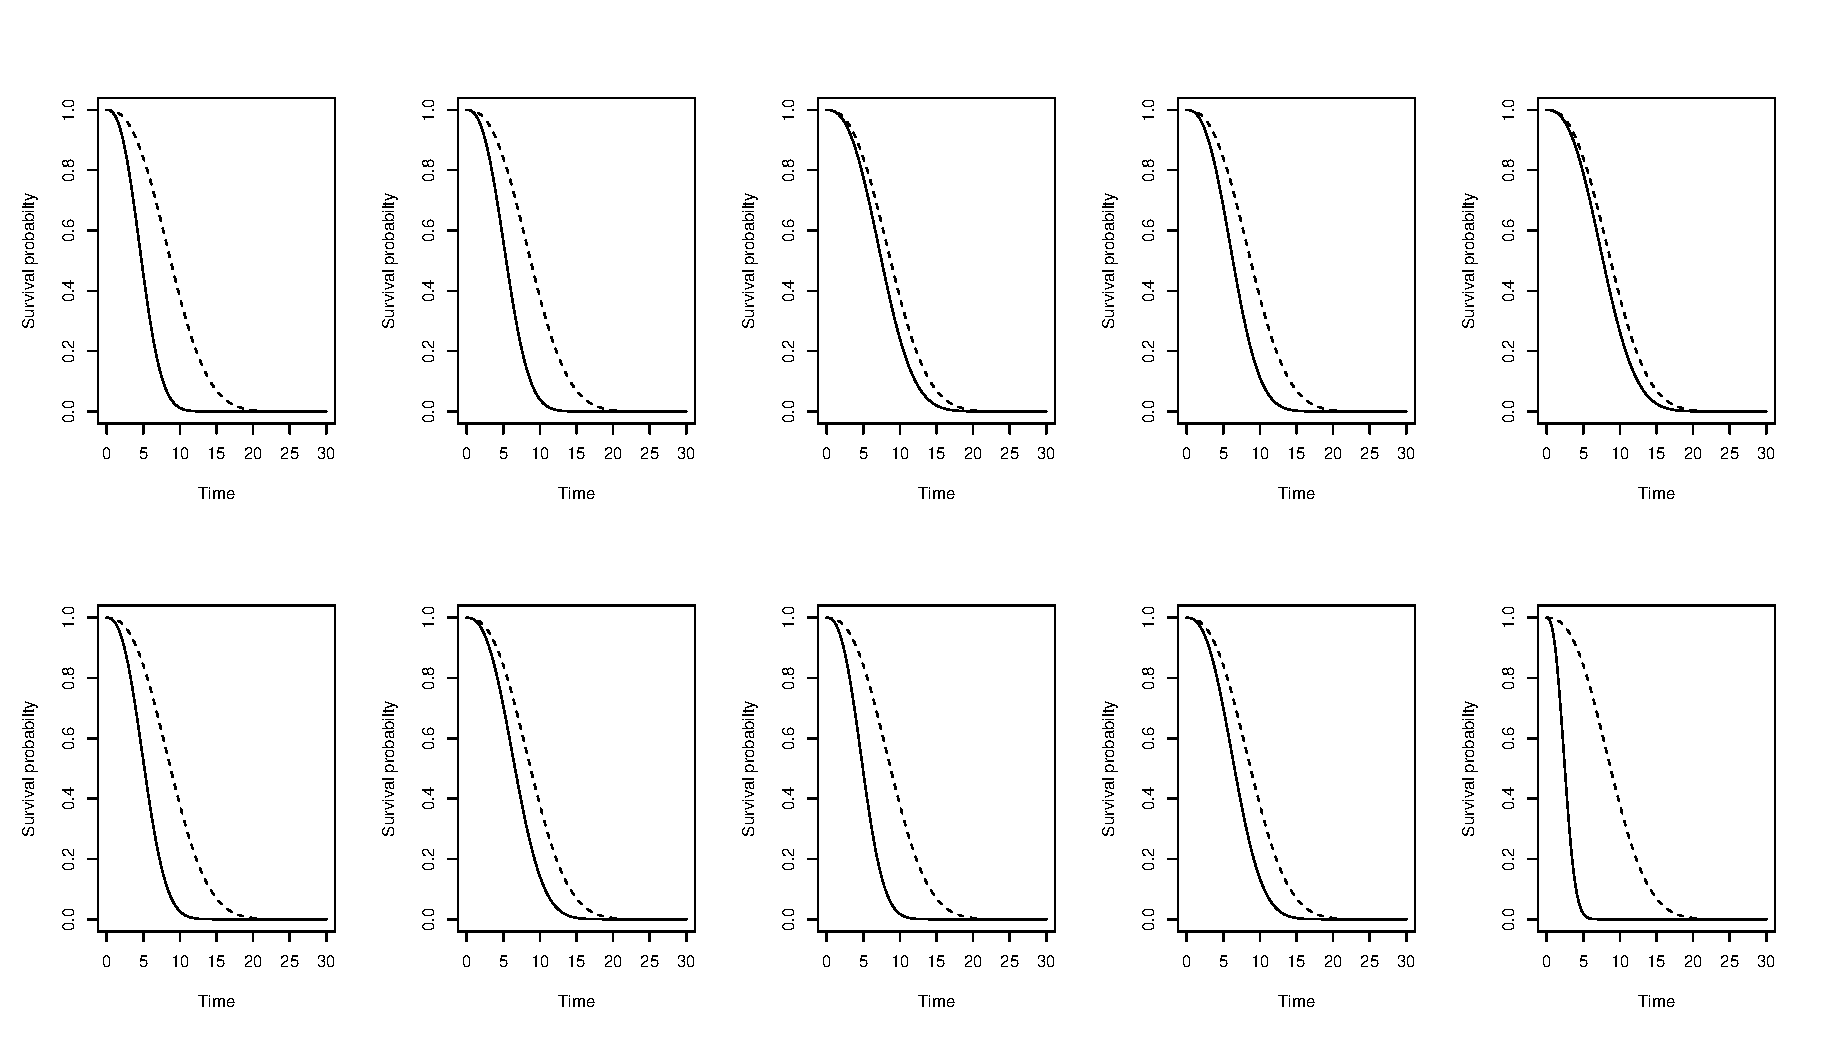
\includegraphics[width=1.05\linewidth]{pics/Countyswise_true_survival_sim_A.eps}
    \caption{The true survival curves for each cluster/county under simulation scenario A. Each plot out of the 10 plots represents the survival curves for a specific county. For each plot, the solid line represents the survival curve for a patient without treatment (Z=0) and all covariates fixed at the respective medians, and the dashed line represents the survival curve for a patient with treatment (Z=1) and all covariates fixed at the respective medians.}
    \label{fig:TruesurvA}
\end{figure}
Figure~1 illustrates the true survival curves for a representative patient in each of the 10 counties. The survival curves are shown for both treated and untreated patients, with all covariates fixed at their median values. From this figure, we observe that the gap between the survival curves, which reflects the treatment effect, varies across counties. Some counties exhibit a substantial difference between treated and untreated survival probabilities, while others show a smaller gap. This variation mimics real-life scenarios, where treatment effects often differ across regions or populations due to varying local factors and patient characteristics.

To estimate the CSPCE, we employ two methods: Cox-PH-PS and AFT-BART-PS, both of which follow a two-step approach. The first step involves estimating the propensity score using BART, which is then used as a covariate in the survival outcome model. In the Cox-PH-PS method, spatial dependencies among counties are explicitly modeled using a Conditional Autoregressive (CAR) structure, accounting for geographic correlations. In contrast, the AFT-BART-PS method assumes independence among observations.

Figure~2 presents the estimated CSPCE for the two methods compared against the true CSPCE across the 10 counties. The results demonstrate that the Cox-PH-PS method closely aligns with the true CSPCE and provides narrower credible intervals, reflecting greater precision. In comparison, the AFT-BART-PS method shows more deviation from the true values and wider credible intervals, particularly in counties where spatial dependencies are significant. This difference in performance is expected, as the outcome model for Cox-PH-PS is correctly specified in this simulation, while AFT-BART-PS does not incorporate spatial associations. This figure demonstrates the ability of each method to capture the true CSPCE and highlights the relative strengths and limitations.


\begin{figure}
    \centering
    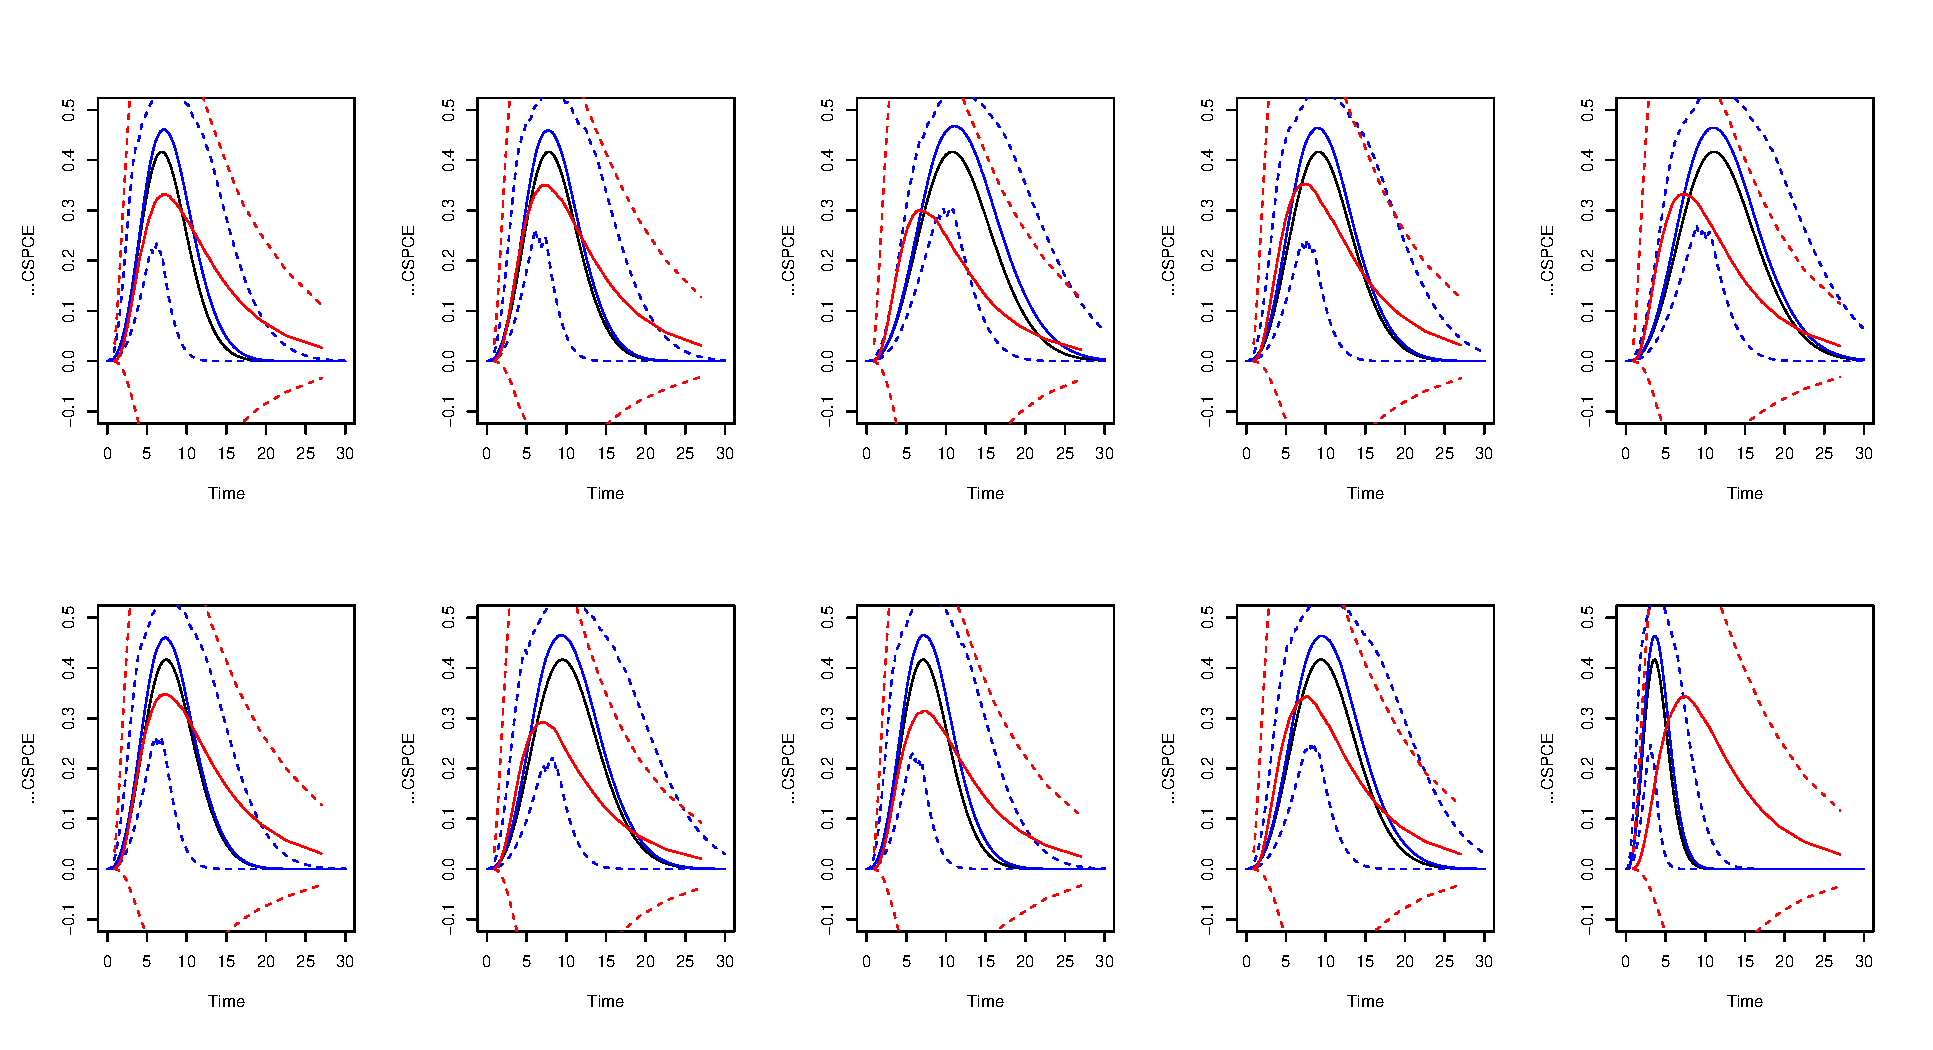
\includegraphics[width=1.05\linewidth]{pics/Countywise_CSPCE_sim_A.eps}
    \caption{Comparison of the true Conditional Survival Probability Causal Effect (CSPCE) and estimates from two methods, Cox-PH-PS and AFT-BART-PS, across 10 counties. Each panel corresponds to a specific county, with covariates fixed at their median values. The black curve represents the true CSPCE for the county, while the red and blue curves depict the CSPCE estimates obtained using AFT-BART-PS and Cox-PH-PS, respectively. Dashed lines of corresponding colors represent the $95\%$ credible intervals for each method, illustrating the uncertainty in the estimates.}
    \label{fig:CSPCE}
\end{figure}

\subsection{Application to the FCR Data}
In the application to the Florida Cancer Registry (FCR) data, we stratify patients into six strata defined by combinations of two races—African American (AA) and Non-African American (WA)—and three cancer stages at diagnosis—Distant (D), Regional (R), and Local (L). This stratification enables us to investigate survival disparities across different race-stage combinations. Key patient-level covariates considered in the analysis include age (continuous), Hormone Receptor (HR) status (categorical: negative/positive), tumor grade (categorical: 1/2/3), Biopsy Delay (BD; categorical: long/short), and Treatment Delay (TD; categorical: long/short).

For each stratum, two separate analyses are performed:
\begin{enumerate}
    \item \textbf{Treatment as Biopsy Delay (BD):} Using BD as the treatment variable while considering other covariates as confounders.
    \item \textbf{Treatment as Treatment Delay (TD):} Using TD as the treatment variable with the remaining covariates as confounders.
\end{enumerate}

These analyses aim to determine whether the causal effects (e.g., ACE, SPCE, CSPCE, CACE) vary across different strata, i.e., by race and cancer stage. By focusing on the impacts of treatment delays, such as TD and BD, the findings can inform targeted interventions to reduce racial disparities in cancer survival and improve overall survival rates.

Furthermore, we will calculate county-specific and conditional average treatment effects to understand how these effects vary geographically. Such insights are essential for developing country-specific policies, guiding resource allocation, and promoting health equity at both the local and state levels.

Finally, we will compare the importance of the treatment factors—Treatment Delay (TD) and Biopsy Delay (BD)—in influencing survival outcomes across the different strata. By examining the causal effects (e.g., CSPCE and CACE) across varying strata and confounder values, we aim to identify whether one treatment has a more significant impact on survival disparities. This comparison will help determine which treatment variable is more critical in improving outcomes for specific patient groups stratified by race and cancer stage. Understanding the comparative importance of TD versus BD not only provides insights into the most impactful areas for intervention but also supports the development of personalized care strategies and the formulation of equitable health policies that address survival disparities effectively.



%%% The skeleton document in the thesis-template folder gives an
%%% example of the "simple" 'references' environment.  In that
%%% document, you must format all of your own references and manage
%%% your own citation styling.  In contrast, this document assumes
%%% that I will be using BibLaTeX to format my references.  I'll be
%%% using the default plain format style, and the bibliographic data
%%% are kept in the file 'myrefs.bib'. This is specified in the
%%% document preamble above.

%%% If using biblatex/biber, then this is the command required
%%% to render the bibliography/references section correctly.

\printbibliography
\end{document}
